%\section{Organización Lógica del Código}

El código del \emph{plugin} se separó en una serie de módulos lógicos que encapsulan y abstraen cada uno una categoría de funcionalidades de la interfaz con TraCI. De esta manera, se logró una separación lógica de las funcionalidades implementadas, y se simplifican futuras extensiones al código. La organización en archivos de éstos módulos puede observarse en la figura \ref{fig:dirtree}, y puede explorarse en línea en el repositorio del proyecto \autocite{pveins_github}.

Cabe notar también que se utilizó el \emph{namespace} \texttt{traci\_api} para agrupar los elementos propios del framework. 

\begin{figure}[tpbh]
    \dirtree{%
        .1 src/.
        .2 plugin.c\DTcomment{Archivo de inicio del \emph{plugin}}.
        .2 TraCIAPI/\DTcomment{Implementación de la API}.
        .3 Constants.h\DTcomment{Constantes utilizadas en el sistema}.
        .3 Exceptions.h\DTcomment{Excepciones propias del framework}.
        .3 Network.\{cpp/h\}\DTcomment{Métodos de interacción con la red vehicular}.
        .3 Simulation.\{cpp/h\}\DTcomment{Métodos de interacción con la simulación vehicular}.
        .3 Subscriptions.\{cpp/h\}\DTcomment{Suscripciones TraCI}.
        .3 TraCIServer.\{cpp/h\}\DTcomment{Módulo principal, manejo de conexiones TraCI}.
        .3 Triggers.\{cpp/h\}\DTcomment{Operaciones disparadas (temporales o situacionales)}.
        .3 Utils.\{cpp/h\}\DTcomment{Funciones auxiliares y de conveniencia}.
        .3 VehicleManager.\{cpp/h\}\DTcomment{Métodos de interacción con vehículos}.
        .2 shawn/\DTcomment{Archivos externos}.
        .3 socket.\{cpp/h\}\DTcomment{Manejo simplificado de \emph{sockets} TCP}.
        .3 storage.\{cpp/h\}\DTcomment{Manejo simplificado de paquetes de datos}.
        .1 veins/.
        .2 paramics-launchd.py\DTcomment{\emph{Script} python de inicio del \emph{framework}}. 
    }
    \caption{Estructura de archivos del código fuente del framework.}
    \label{fig:dirtree}
\end{figure}

\begin{figure}[tpbh]
    \centering
    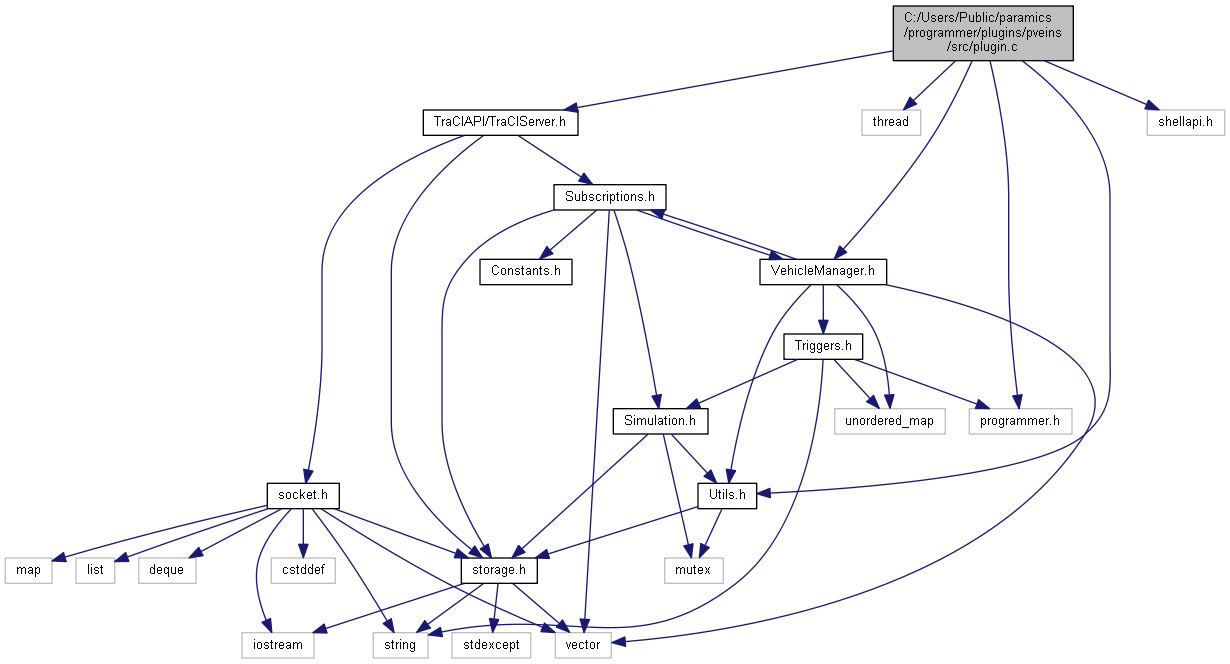
\includegraphics[angle=90, origin=c, height=0.6\textheight]{figuras/plugin_dependency_graph.png}
    \caption{Gráfico de dependencia entre los componentes del \emph{framework}.}
    \label{fig:dependencygraph}
\end{figure}

A continuación, se presenta en detalle la implementación de cada uno de los módulos del software. Se discutirán decisiones de diseño e implementación, además de consideraciones ligadas al funcionamiento de TraCI.